\documentclass{beamer}
\usepackage[hangul]{kotex}
\usepackage{graphicx}
\usepackage{graphbox}
\usepackage{href-ul}
\usepackage{verbatim}
\usetheme{Copenhagen}
\usecolortheme{beaver}
\usefonttheme{serif}
\SetHangulFonts{nanummj}{nanummj}{nanummj}

\definecolor{bgcolor}{RGB}{236, 220, 220}
\definecolor{fgcolor}{RGB}{190, 20, 20}
\setbeamercolor{title}{bg=bgcolor, fg=fgcolor}
\setbeamercolor{frametitle}{bg=bgcolor, fg=fgcolor}

\setbeamertemplate{section in toc}[circle]
\setbeamertemplate{subsection in toc}[square]
\setbeamertemplate{itemize items}[circle]
\setbeamertemplate{enumerate items}[circle]

\beamertemplateheadempty
\beamertemplatefootempty
\beamertemplatenavigationsymbolsempty

\newcommand{\spacing}{\hspace{0.3em}}
\newcommand{\eg}{\textbf{eg}}
\newcommand{\imgascii}{\textbf{img2ascii}}
\newcommand{\libpng}{\textbf{libpng}}
\newcommand{\Eigen}{\textbf{Eigen}}
\newcommand{\tonebased}{\textbf{tone-based}}
\newcommand{\structurebased}{\textbf{structure-based}}


\title{AAC - Ascii Art Converter}
\author{No More Double \\ 조다니엘, 박준영}
\date{\today}
\institute{Sogang University \\ CSE2035/AIE2051}

\begin{document}

\section{}
\begin{frame}{}
	\titlepage
	\begin{figure}
		\vspace{-1em}
		
\includegraphics[width=2cm]{sogang_university_logo}
		\vspace{1em}
	\end{figure}
\end{frame}

\section{}
\begin{frame}{}
	\frametitle{목차}
	\tableofcontents
\end{frame}

\section{왜 만들었는가?}
\begin{frame}{}
	\frametitle{왜 만들었는가?}
	\begin{itemize}
		\item AAC(악)이라는 이름이 너무 찰져서
		\item YouTube에서 donut.c라는 아스키 아트를 봤는데 멋있어서\footnote{\href{https://www.youtube.com/watch?v=DEqXNfs\_HhY}{\footnotesize{https://www.youtube.com/watch?v=DEqXNfs\_HhY}}}
	\end{itemize}
	\begin{figure}
		\centering
		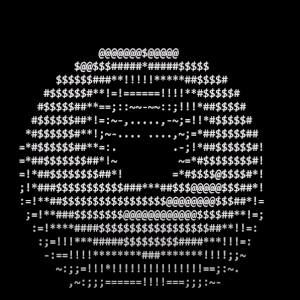
\includegraphics[width=4.5cm, height=4.5cm]{donut.png}
	\end{figure}
\end{frame}

\section{무엇으로 만들었는가?}
\begin{frame}{}
	\frametitle{무엇으로 만들었는가?}
	\begin{enumerate}
		\item 자체 제작 라이브러리: \eg
		\item 메인 루틴: \imgascii
		\item 기타: GitHub, Valgrind, ...
	\end{enumerate}
\end{frame}

	\subsection{\eg}
	\begin{frame}{}
		\frametitle{\eg}
		\textbf{E}asy pn\textbf{G} \\
		\libpng \spacing + \Eigen으로 구성한 자체 제작 라이브러리 \\
		이미지 입출력, 변환, 연산 등에 필요한 클래스를 내장
		\vspace{1em}
		\begin{itemize}
			\item egLoader: 이미지 입출력
			\item egMath: 변환에 필요한 연산 내장 \\ (convolution, Bhattacharyya 거리)
			\item egProcessing: 이미지 변환 \\ (회색조, 흑백, blur, Suzuki, erode, dilate, grassfire)
			\item egGeometry: 외적, 내적, norm 및 거리 계산
			\item egTrace: 이미지 벡터화
		\end{itemize}
	\end{frame}

	\subsection{\imgascii}
	\begin{frame}{}
		\frametitle{\imgascii}
		\eg \spacing 라이브러리를 활용하여 이미지를 처리하는 메인 루틴 \\
		\tonebased \spacing 방식과 \structurebased \spacing 방식으로 나뉨
		\begin{figure}
			(\tonebased \spacing 방식 결과물 사진 한 장, \structurebased \spacing 방식 결과물 사진 한 장 넣기)
		\end{figure}
	\end{frame}

	\subsection{기타}
	\begin{frame}{}
		\frametitle{기타}
		\begin{itemize}
			\item GitHub: 소스 코드 버전 관리 플랫폼
			\begin{figure}
				
\includegraphics[width=3cm, height=2cm]{GitHub1.png}
				\hspace{1em}
				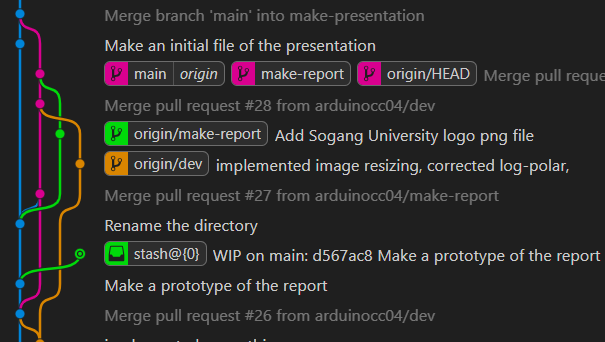
\includegraphics[width=3cm, height=2cm]{GitHub2.png}
			\end{figure}
			\item Valgrind: 메모리 누수 탐지 라이브러리
			\begin{figure}
				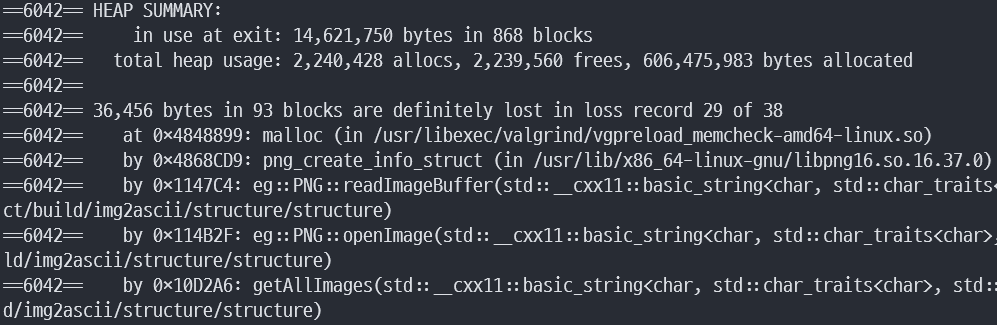
\includegraphics[width=8cm, height=3cm]{Valgrind.png}
			\end{figure}
		\end{itemize}
	\end{frame}

\section{어떻게 동작하는가?}
\begin{frame}{}
	\frametitle{어떻게 동작하는가?}
	\begin{itemize}
		\item \tonebased \spacing 방식 - easy
		\item \structurebased \spacing 방식 - \underline{\textbf{DIFFICULT}}
	\end{itemize}
\end{frame}

	\subsection{\tonebased \spacing 방식}
	\begin{frame}{}
		\frametitle{\tonebased \spacing 방식}
		\begin{enumerate}
			\item 이미지를 3차원 텐서 $ ( width, height, rgba ) $ 형태로 저장
			\item 각 픽셀별 red, green, blue 값의 평균을 구하여 밝기 도출
			\item 밝기 정보를 이용하여 이미지를 회색조로 변환
			\item 밝기에 해당하는 아스키 문자를 출력
		\end{enumerate}
	\end{frame}
	\begin{frame}
		\frametitle{결과}
			\begin{figure}
			\centering
			\includegraphics[align=c, width=5cm, height=7cm]{Tree.png}
			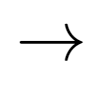
\includegraphics[align=c, width=0.5cm, height=0.5cm]{Rightarrow.png}
			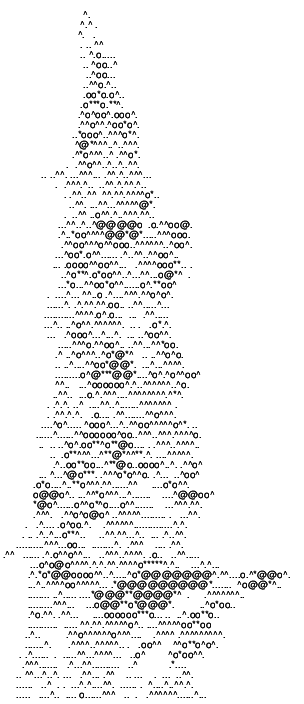
\includegraphics[align=c, width=5cm, height=8cm]{TreeToneBased.png}
			\end{figure}
	\end{frame}

	\subsection{\structurebased \spacing 방식}
	\begin{frame}{}
		\frametitle{\structurebased \spacing 방식}
		\begin{enumerate}
			\item 이미지 저장
			\item 회색조 변환
			\item Binary 변환
			\item 외곽선의 선분 근사
			\item 아스키 문자로 최적화
		\end{enumerate}
	\end{frame}
	\begin{frame}[fragile]
		\frametitle{이미지 저장}
			이미지를 3차원 텐서 $ ( height, width, rgba ) $ 형태로 저장
			\line(1,0){1000}
			\begin{verbatim}
				using Image = Eigen::Tensor<png_byte, 3>;
				
				image.dimensions()[0]: height
				image.dimensions()[1]: width

				image(i, j, 0): red
				image(i, j, 1): green
				image(i, j, 2): blue
				image(i, j, 3): alpha
			\end{verbatim}
	\end{frame}
	\begin{frame}{}
		\frametitle{회색조 변환}
		\begin{itemize}
			\item 색조 이미지를 회색조로 변환
			\item red, green, blue 값의 평균을 밝기로 치환
			\item tone-based 방식과 동일
		\end{itemize}
		\vspace{2em}
		\centering
		$ \displaystyle \frac{red + green + blue}{3} = brightness $
	\end{frame}
	\begin{frame}{}
		\frametitle{Binary 변환}
		\begin{enumerate}
			\item Gaussian-blur $ \rightarrow $ Binary
			\begin{itemize}
				\item $ 3 \times 3 $ Gaussian 필터를 이용해 convolution 연산을 적용 \\
				\item 이미지를 흐리게 처리
			\end{itemize}
		\end{enumerate}
		\begin{figure}
			\centering
			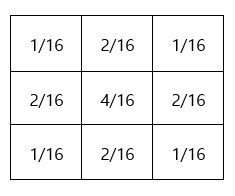
\includegraphics[width=3cm, height=2.5cm]{GaussianFilter.png} \\
			\vspace{-0.5em}
			\tiny{Gaussian 필터}
		\end{figure}
	\end{frame}
	\begin{frame}{}
		\frametitle{Binary 변환}
		\begin{itemize}
			\item Convolution 연산
		\end{itemize}
		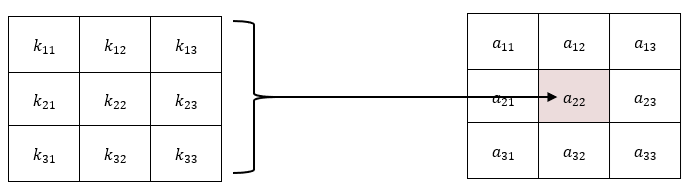
\includegraphics[width=10cm, height=2.5cm]{Convolution.png}
		\centering
		$ \displaystyle a_{22} = \sum_{i = 1}^{3} \sum_{j = 1}^{3} a_{ij} * k_{ij} $
	\end{frame}
	\begin{frame}{}
		\frametitle{Binary 변환}
		\begin{enumerate}
			\setcounter{enumi}{1}
			\item Binary $ \rightarrow $ Morphology
			\begin{itemize}
				\item erosion: 범위에 0이 존재하면 0으로 변환 \\
				\vspace{0.5em}
				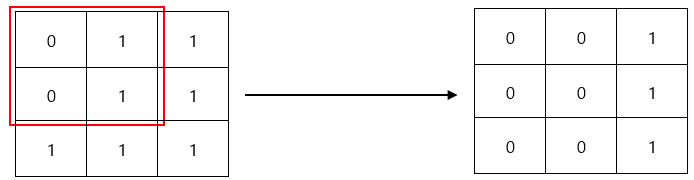
\includegraphics[width=8cm, height=2cm]{Erosion.png}
				\item dilation: 범위에 1이 존재하면 1로 변환 \\
				\vspace{0.5em}
				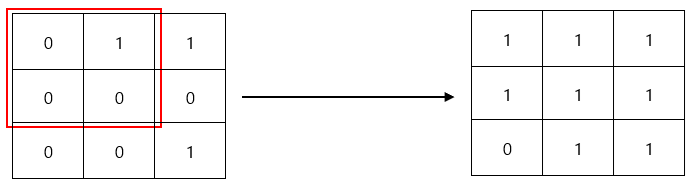
\includegraphics[width=8cm, height=2cm]{Dilation.png}
			\end{itemize}
		\end{enumerate}	
	\end{frame}
	\begin{frame}{}
		\frametitle{외곽선의 선분 근사}
		\begin{enumerate}
			\item Suzuki 알고리즘을 이용하여 외곽선을 추출
			\item 자체 제작한 CW 정렬 알고리즘을 이용하여 외곽선을 선분으로 분할
		\end{enumerate}	
	\end{frame}
	\begin{frame}{}
		\frametitle{외곽선의 선분 근사}
		CW 정렬 알고리즘
		\line(1,0){1000}
		\begin{enumerate}
			\item 왼쪽 위 $(0, 0)$부터 오른쪽 아래 $(H, W)$ 방향으로 행렬의 각 원소를 검사한다. \label{CW1}
			\item 현재 픽셀의 왼쪽 아래에 위치한 픽셀부터 시계 반대 방향으로 자신과 같은 외곽선에 속한 픽셀을 찾는다. \label{CW2}
			\item 연결된 픽셀을 순차적으로 탐색하며 연결된 픽셀이 더 이상 없을 때까지 스택에 픽셀의 좌표를 넣는다.
		\end{enumerate}
	\end{frame}
	\begin{frame}{}
		\frametitle{외곽선의 선분 근사}
		\begin{enumerate}
			\setcounter{enumi}{3}
			\item 스택을 뒤집는다. (CCW $ \rightarrow $ CW)
			\item \ref{CW2}에서 얻은 픽셀의 시계 반대 방향에 위치한 다음 픽셀부터 시계 반대 방향으로 탐색을 시작한다.
			만약 기존에 방문한 픽셀밖에 없거나, 같은 외곽선에 속한 픽셀을 찾을 수 없다면 \ref{CW1}로 되돌아간다.
		\end{enumerate}
	\end{frame}
	\begin{frame}{}
		\frametitle{아스키 문자로 최적화}
		\begin{enumerate}
			\item Cohen-Sutherland 알고리즘을 사용하여 길이가 긴 선분을 일정한 간격의 그리드로 분할
			\item Simulated annealing(담금질 기법): 임의의 정점을 조금씩 움직이면서 Bresenham's line algorithm을 사용해 그림을 새로 그림
			\item 새로 그린 이미지가 아스키 아트로 더 잘 표현되는 결과물로 변화하였는지 확인
		\end{enumerate}	
	\end{frame}
	\begin{frame}{}
		\frametitle{아스키 문자로 최적화}
		\begin{enumerate}
			\setcounter{enumi}{3}
			\item 주어진 그리드에 어떤 문자가 가장 잘 대응되는지 판단하기 위하여 좌표계를 log-polar coordinate로 변환한 후 히스토그램을 만듦
			\item 히스토그램 간의 Bhattacharyya 거리를 비교하여 최적의 아스키 문자를 판단
		\end{enumerate}
		\vspace{1em}
		Bhattacharyya 거리: \\
		\vspace{0.5em}
		\centering
		$ \displaystyle d(H_1,H_2) = \sqrt{1 - \frac{1}{\sqrt{\bar{H_1} \bar{H_2} N^2}} \sum_I \sqrt{H_1(I) \cdot H_2(I)}} $
		\vspace{0.5em}
		\begin{itemize}
			\item 히스토그램을 전체 크기로 나누어 합이 1인 확률분포로 변형
			\item 확률분포화된 히스토그램의 유사도를 계산
		\end{itemize}
	\end{frame}

	\begin{frame}{}
		\frametitle{결과}
		\begin{figure}
			\centering
			(처음 input 사진 한 장 $ \rightarrow $ 아스키 아트 사진 한 장)
		\end{figure}
	\end{frame}
	\begin{frame}{}
		\frametitle{참고 자료}
		\begin{enumerate}
			\item 자료 1
			\item 자료 2
			\item 자료 3
		\end{enumerate}
		(인용 양식 지켜서 쓰면 교수님 호감 $ \rightarrow $ 대학원생으로 바로 납치)
	\end{frame}

	\begin{frame}
		\centering
		감사합니다.
	\end{frame}

\end{document}
